\subsection{BigNetSim Design and Internals}
\begin{figure}[!t]
\centering  
  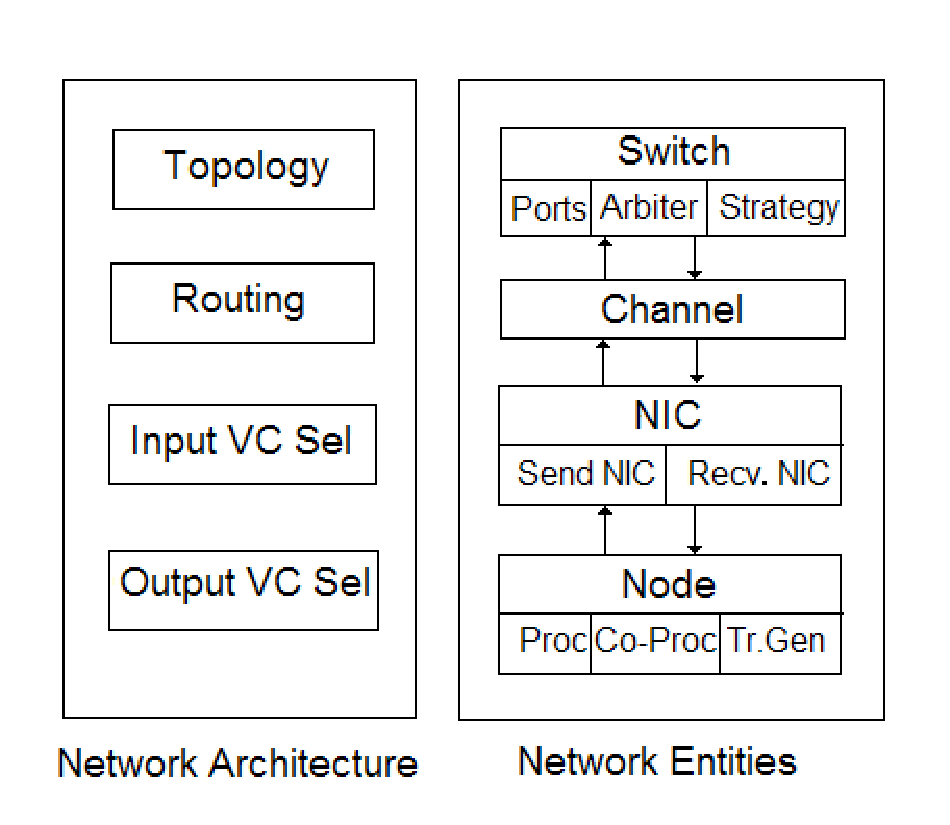
\includegraphics[width=3.2in]{figures/detailedsim_newer}
{\sffamily\bfseries\small \caption{BigNetSim conceptual model\label{fig:detailedsim_model}}}
\end{figure}

This section focuses on the interconnection network simulation.
The entities that form an interconnection network are:
\begin{itemize}
\item {\it switch:} A switch decides the routing on a packet. Switches could be
input buffered or output buffered. The former are implemented as individual posers
per port of each switch while the latter are implemented as a poser per switch.
In an {\it Input Buffered (IB)} switch, a packet in a switch is stored at the input 
port until its next route is decided and leaves the switch if it finds 
available space on the next switch in the route.
While in an {\it Output Buffered (OB)} switch, a packet in a switch decides beforehand 
on the next route to take and is buffered at the output port until space is
available on the next switch along the route.
Switches are modeled in much detail. Ports, buffers and
virtual channels at ports to avoid head-of-the-line blocking are
modeled.  Hardware collectives are implemented on the switch to
enable broadcasts, multicasts and other collective operations
efficiently. These are configurable and can be used if the system
being simulated supports them. We also support configurable
strategies for arbitration, input virtual channel selection and output
virtual channel selection. The configurability of the switch
provides a flexible design, satisfying the requirements of
a large number of networks.

\item {\it network card:} Network cards packetize and unpacketize messages.
A NIC is implemented as two posers. The sending and receiving entities in a
NIC are implemented as separate posers. A NIC is attached to each node.
\item {\it channel:} These are modeled as posers and connect a NIC to a switch
or a switch to another switch.
\item {\it compute node:} Each compute node connects to a network interface card.
A compute node simulates execution of entry methods on it. It is also attached
to a message traffic generator, which is used when only an interconnection
network is being simulated. This traffic generator can generate any message
pattern on each of the compute nodes.
The traffic generator can send
point-to-point messages, reductions, multicasts, broadcasts and other
collective traffic.  It supports k-shift, ring, bit-transpose,
bit-reversal, bit-complement and uniform random traffic.
These are based on common communication patterns found in
real applications. The frequency of message generation is determined
by a uniform or Poisson distribution.
\end{itemize}


\subsection{Topology, Routing and Virtual Channel Selection}
Topology, Routing strategies and input and output virtual channel selection
strategies need to be decided for any inter-connection network. Once we
have all of these in place we can simulate an inter-connection network.

\subsubsection{Topology}
For every architecture one wants to design, a topology file has to written
which defines a few basic functions for that particular topology.
These are:

\function{void getNeighbours(int nodeid, int numP);}
\index{getNeighbours}
\desc{This is called initially for every switch and this populates the
data structure {\it next} in a switch which contains the connectivity
of that switch. The switch specified by {\it switch} has {\it numP} ports.}

\function{int getNext(int portid, int nodeid, int numP)}
\index{getNext}
\desc{Returns the index of the switch/node that is connected to the
switch {\it nodeid}, at {\it portid}. The number of ports this node has is {\it numP}.}

\function{int getNextChannel(int portid, int nodeid, int numP)}
\index{getNextChannel}
\desc{Returns the index of the channel that is connected to the
switch {\it nodeid}, at {\it portid}. The number of ports this node has is {\it numP}.}

\function{int getStartPort(int nodeid, int numP, int dest)}
\index{getStartPort}
\desc{Return the index of the port that is connected to this compute node from a switch}

\function{int getStartVc()}
\index{getStartVc}
\desc{Returns the index of the first virtual channel (mostly 0).}

\function{int getStartSwitch(int nodeid)}
\index{getStartSwitch}
\desc{Returns the index of the node/switch that is connected to the first port}

\function{int getStartNode()}
\index{getStartNode}
\desc{Returns the index of the first node. Each poser has a separate index, 
irrespective of the type of the poser.}

\function{int getEndNode()}
\index{getEndNode}
\desc{Returns the index of the last node.}


\subsubsection{Routing}
Routing strategy needs to be specified for every interconnection network.
There is usually at least one routing strategy that needs to be defined
for every topology, Usually we have many more. The following functions need
to be defined for every routing strategy.

\function{int selectRoute(int current, int dest, int numP, Topology* top, Packet *p, map<int,int> \&bufsize, unsigned short *xsubi)}
\index{selectRoute}
\desc{Returns the portid that should be taken on switch {\it current} if the destination
is {\it dest}. The number of ports on a switch is {\it numP}. We also pass the pointer 
to the topology and to the Packet.}

\function{int selectRoute(int current, int dest, int numP, Topology* top, Packet *p, map<int,int> \&bufsize, map<int,int> \&portContention, unsigned short *xsubi)}
\index{selectRouteCont}
\desc{Returns the portid that should be taken on switch {\it current} if the destination
is {\it dest}. The number of ports on a switch is {\it numP}. We also pass the pointer 
to the topology and to the Packet. {\it Bufsize} is the state of the ports in
a switch, i.e. how many buffers on each port are full, while {\it portContention}
is used to give priority to certain ports, when more options are available.}

\function{int expectedTime(int src, int dest, POSE\_TimeType ovt, POSE\_TimeType origOvt, int length, int *numHops)}
\index{expectedTime}
\desc{Returns the expected time for a packet to travel from {\it src} to {\it dest},
when the number of hops it will need to travel is {\it numHops}.}

\function{int convertOutputToInputPort(int id, Packet *p, int numP, int *next)}
\index{convertOutputToInputPort}
\desc{Translate this output port to input port on the switch this port is
connected to.}


\subsubsection{Input Virtual Channel Selection}
For every switch, we need to know the mechanism it uses to choose input virtual channel.
There are a few different input virtual channel selection strategies, and a switch
can choose among them. Each should implement the following function.

\function{int selectInputVc(map<int,int> \&availBuffer, map<int,int> \&request, map<int,vector<Header> > \&inBuffer, int globalVc, int curSwitch)}
\index{selectInputVc}
\desc{Returns the input virtual channel to be used depending on the strategy and
the input parameters.}


\subsubsection{Output Virtual Channel Selection}
For every switch, we need to know the mechanism it uses to choose output virtual channel.
There are a few different output virtual channel selection strategies, and a switch
can choose among them. Each should implement the following function.

\function{int selectOutputVc(map<int,int> \&bufsize, Packet *p, int unused)}
\index{selectOutputVc}
\desc{Returns the output virtual channel to be used depending on the strategy and
the input parameters.}

